%%%%%%%%%%%%%%%%%%%%%%% file template.tex %%%%%%%%%%%%%%%%%%%%%%%%%
%
% This is a template file for Web of Conferences Journal
%
% Copy it to a new file with a new name and use it as the basis
% for your article
%
%%%%%%%%%%%%%%%%%%%%%%%%%% EDP Science %%%%%%%%%%%%%%%%%%%%%%%%%%%%
%
%%%\documentclass[option]{webofc}
%%% "twocolumn" for typesetting an article in two columns format (default one column)
%
\documentclass{webofc}
\usepackage[varg]{txfonts}   % Web of Conferences font
%
% Put here some packages required or/and some personnal commands
%
%
\begin{document}
%
\title{ServiceX}
%
% subtitle is optionnal
%
\subtitle{A Distributed, Caching, Columnar Data Delivery Service}

\author{\firstname{B.} \lastname{Galewsky}\inst{1}\fnsep\thanks{\email{bengal1@illinois.edu}} \and
        \firstname{R.} \lastname{Gardner}\inst{2}\fnsep\thanks{\email{rwg@uchicago.edu}} \and
        \firstname{L.} \lastname{Gray}\inst{5}\fnsep\thanks{\email{Lindsey.Gray@cern.ch}} \and
        \firstname{M.} \lastname{Neubauer}\inst{1}\fnsep\thanks{\email{msn@illinois.edu}} \and
        \firstname{J.} \lastname{Pivarski}\inst{3}\fnsep\thanks{\email{pivarski@princeton.edu}} \and
        \firstname{M.} \lastname{Proffitt}\inst{4}\fnsep\thanks{\email{masonlp@uw.edu}} \and
        \firstname{I.} \lastname{Vukotic}\inst{2}\fnsep\thanks{\email{ivukotic@uchicago.edu}} \and
        \firstname{G.} \lastname{Watts}\inst{4}\fnsep\thanks{\email{gwatts@uw.edu}} \and
        \firstname{M.} \lastname{Weinberg}\inst{2}\fnsep\thanks{\email{mweinberg@uchicago.edu}}
}

A: University of Illinois at Urbana-Champaign, B: The University of Chicago,
C: Princeton University, D: University of Washington, E: Fermilab

\institute{University of Illinois at Urbana-Champaign
\and
           The University of Chicago
\and
           Princeton University
\and
           University of Washington
\and
           Fermilab
          }

\abstract{%
  We will describe a component of the Intelligent Data Delivery Service being developed in
  collaboration with IRIS-HEP and the LHC experiments. ServiceX is an experiment-agnostic service
  to enable on-demand data delivery specifically tailored for nearly-interactive vectorized
  analysis. This work is motivated by the data engineering challenges posed by HL-LHC data volumes
  and the increasing popularity of python and Spark-based analysis workflows.
  \medskip
  
  ServiceX gives analyzers the ability to query events by dataset metadata. It uses containerized
  transformations to extract just the data required for the analysis. This operation is collocated
  with the data lake to avoid transferring unnecessary branches over the WAN. Simple filtering
  operations are supported to further reduce the amount of data transferred.
  \medskip
  
  Transformed events are cached in a columnar datastore to accelerate delivery of subsequent
  similar requests. ServiceX will learn commonly related columns and automatically include them in
  the transformation to increase the potential for cache hits by other users.
  \medskip
  
  Selected events are streamed to the analysis system using an efficient wire protocol that can be
  readily consumed by a variety of computational frameworks. This reduces time-to-insight for
  physics analysis by delegating to ServiceX the complexity of event selection, slimming,
  reformatting, and streaming.
}
%
\maketitle
%
\section{Introduction}
\label{sec:intro}
Data organization in HEP experiments often follows a standard workflow, starting from raw detector
data or simulated data, which is processed by reconstruction algorithms into higher-level physics
objects. This reconstructed data is then used as input to analysis software to produce physics
insights. While the reconstruction step is typically performed centrally and a standardized output
is made available to the entire collaboration, the analysis software is often written by small
groups or individual analysts, with idiosyncratic selection and processing steps.

\section{ServiceX overview}
\label{sec:overview}
Join us here \cite{RefServiceX}.

\subsection{ServiceX features}
\label{subsec:features}
Don't forget to give each section, subsection, subsubsection, and
paragraph a unique label (see Sect.~\ref{sec:overview}).

\subsection{Simple transform requests}
\label{subsec:requests}

\subsection{Transformation output}
\label{subsec:output}

\section{ServiceX implementation}
\label{sec:implement}

\subsection{ServiceX architecture}
\label{subsec:architect}

\subsection{Python transformers}
\label{subsec:pyTransform}

\section{What's next?}
\label{sec:whatNext}
Version 1 is available today at \cite{RefServiceX}.

\subsection{Version 2--with C++ transformers}
\label{subsec:v2}

\subsection{Selection code}
\label{subsec:select}

For one-column wide figures use syntax of figure~\ref{fig-1}
\begin{figure}[h]
% Use the relevant command for your figure-insertion program
% to insert the figure file.
\centering
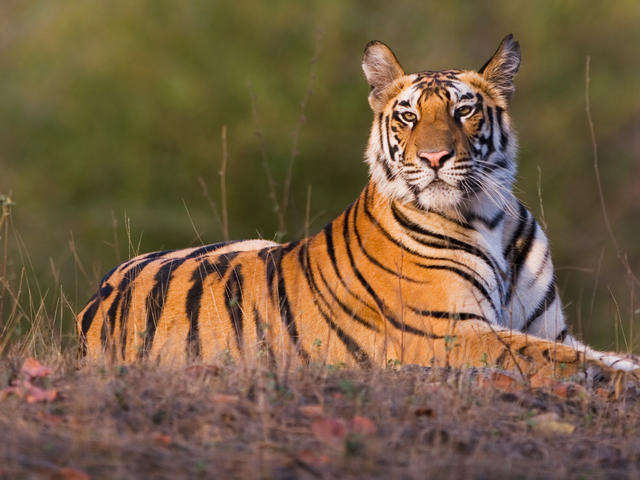
\includegraphics[width=5cm,clip]{tiger}
\caption{Please write your figure caption here}
\label{fig-1}       % Give a unique label
\end{figure}

For tables use syntax in table~\ref{tab-1}.
\begin{table}
\centering
\caption{Please write your table caption here}
\label{tab-1}       % Give a unique label
% For LaTeX tables you can use
\begin{tabular}{lll}
\hline
first & second & third  \\\hline
number & number & number \\
number & number & number \\\hline
\end{tabular}
% Or use
\vspace*{5cm}  % with the correct table height
\end{table}
%
% BibTeX or Biber users please use (the style is already called in the class, ensure that the "woc.bst" style is in your local directory)
% \bibliography{name or your bibliography database}
%
% Non-BibTeX users please use
%
\begin{thebibliography}{}
%
% and use \bibitem to create references.
%
% \bibitem{RefJ}
% Format for Journal Reference: Journal Author, Journal \textbf{Volume}, page numbers (year)
% \bibitem{RefB}
% Format for books: Book Author, \textit{Book title} (Publisher, place, year) page numbers
\bibitem{RefServiceX}
\textit{https://github.com/ssl-hep/ServiceX}
\bibitem{RefEventStreams}
\textit{https://ibm.github.io/event-streams/about/key-concepts/}
\end{thebibliography}

\end{document}

% end of file template.tex

<div id='footer'><table width='100%'><tr><td class='right'><a href='http://fusioninventory.org/'><span class='copyright'>FusionInventory 9.1+1.0 | copyleft <img src='/glpi/plugins/fusioninventory/pics/copyleft.png'/>  2010-2016 by FusionInventory Team</span></a></td></tr></table></div>
